%5000 words
\documentclass[10pt, letterpaper]{report}       % Set document class
\usepackage[utf8x]{inputenc}                    % Used to encode document
\usepackage{subfiles}                           % Allows sub files

% ================================================
%           PACKAGES
% ================================================

% === GENERAL ===
\usepackage[english]{babel}     % Set language of document
\usepackage{hyperref}			% Allows hyperlink references
\usepackage[toc]{appendix}	    % Improves appendix behaviour
\usepackage{url}				% Improves URL behaviour
\usepackage[bottom]{footmisc}   % Set footnote style
%\setlength\parindent{0pt}      % Set indent first line paragraph
\usepackage{parskip}            % Creates vertical space between paragraphs
%\usepackage{lipsum}            % Enables lipsum text fillers

% === MATH ===
\usepackage{amsmath}            % Align equations
\usepackage{amssymb}            % Allow different math fonts
%\usepackage{siunitx}           % Standardizes appearance of numbers and units

% To prevent annoying spacing \left{(} and \right{)} https://tex.stackexchange.com/questions/2607/spacing-around-left-and-right
%%%\let\originalleft\left
%%%\let\originalright\right
%%%\renewcommand{\left}{\mathopen{}\mathclose\bgroup\originalleft}
%%%\renewcommand{\right}{\aftergroup\egroup\originalright}

% === CODE ===
\usepackage{listings}           % For advanced code
\usepackage{minted}             % Python code
\usepackage[T1]{fontenc}        % < and > visible in code (icm 'minted' package)

% === FIGURES & TABLES ===
\usepackage{graphicx}           % Allows use of images
\usepackage[format=plain, labelfont={it}, textfont=it]{caption}   % Set caption style
\usepackage{wrapfig}			% Allows wrapping of text around figures
\usepackage{float}				% Improves image placement
\usepackage{subfigure}          % Allows subfigures
%\usepackage{sidecap}           % Allows Figure captions on the side
%\usepackage{subcaption}        % Allows subcaptions within figures
%\usepackage{lscape}            % Allows rotated tables
\usepackage{booktabs}			% Allows professional tables
\usepackage{tabu}				% Powerful table environment
\usepackage{tabularx}
\usepackage{multirow}           % Multiple rows in tables

% === SYMBOLS & TEXT STYLES ===
\usepackage{gensymb}            % Symbols degree, Celsius, etc.
%\usepackage{soul}              % Underlining, striking out, etc.
%\usepackage{libertine}         % Enables extra fonts
\usepackage{comment}            % Allows to comment chunks of text
\usepackage{epigraph}           % Allows epigraphs

% === CITATIONS & BIBLIOGRAPHY ===
%\usepackage{natbib}            % Set citation style
\bibliographystyle{apalike}     % Set bibliography style

% === SET PAGE SIZE & MARGINS ===
% a4: 595 pt x 842 pt
\usepackage{geometry}           % Enables to set margins
\geometry{a4paper, top=25mm, bottom=25mm}              % Set paper size
\voffset = 0pt                  % Set offset top
\textheight = 650pt             % Set page-text length
\footskip = 45pt   % Set foot distance

% === SET HEADER & FOOTER ===
\usepackage{fancyhdr}			% Enables fancy header of page
\pagestyle{fancy}               % Set page style
\fancyhf{}
\lhead{}
\rhead{}
\lfoot{\small \color{JADSred} TUe \color{black}- Technische Universiteit Eindhoven}
\rfoot{}
\cfoot{\thepage}
\renewcommand{\headrulewidth}{0pt}

% === SET CHAPTER & SECTION STYLE ===
\usepackage{titlesec}           % Customize style chapters and sections
\titleformat{\chapter}{\LARGE\normalfont\bfseries}{\thechapter}{1em}{}
\titlespacing*{\chapter}{0pt}{0pt}{20pt}

% === COLORS ===
\usepackage{color}                          % Allows basic colors
\usepackage{xcolor}                         % Allows more colors
\definecolor{purple}{HTML}{cbcefb}          % Define own color
\definecolor{JADSred}{HTML}{b32b0a}         % Define own color
\definecolor{orange}{HTML}{ffce93}          % Define own color
\definecolor{lightgray}{HTML}{d3d3d3}       % Define own color
\definecolor{codeyellow}{HTML}{ffecb2}      % Background code


%=================================================
\begin{document}

% ================================================
%           TITLE PAGE
% ================================================
\begin{titlepage}

\thispagestyle{empty}

\begin{center}
	\begin{figure}[H]
		\centering
		
\includegraphics[width=0.4\textwidth]{Fig/jads_logo.png}
	\end{figure}
	\huge{JADS \\ JM0140-M-6 - Data Engineering\\
	\line(1,0){300}\\[2cm]
    \huge{\textbf{Report\\
     \underline{\textbf{Assignment 1}}\\
    
    }}\\[1.5cm]
    \huge{\textit{Group 12}}\\[1.5cm]
\end{center}

\begin{table}[H]
\Large
\centering
\begin{tabular}{l l}

% names here
Krzysztof Wieśniakowski & 2124849 \\
Kyriakos Koukiadakis & 2074817\\
Xavier Paulus & 2047901\\
Vishal Sehgal & 2109374 \\
Chigozie Ifepe & 2109365\\

\end{tabular}
\end{table}

\begin{center}
\begin{Large}
\centering
% Supervisor1:\\

% Name1\\\\

% Supervisor 2::\\

% Name2


\vspace{20pt}
\end{Large}
\end{center}

\begin{center}
\begin{Large}
\centering
\today \\
\end{Large}
\end{center}

\end{titlepage}

% ================================================
%           CHAPTERS
% ================================================

\tableofcontents

\vfill
The code is available in our repository: 
\newline \url{https://github.com/krzysztof99xd/DE2023Assignment1} 

The Jupyter notebook and the data we used are available at:
\newline \url{https://www.kaggle.com/code/x1wello1x/prediction-of-strokes}


\chapter{{Overview of the ML Application}}
\label{ch:chapter1}
\section{ML application goals}

The ML application built for this assignment is created to predict whether someone is likely to have a stroke attack or not. Every year 47,000 people suffer from a stroke in the Netherlands. Over the next ten years, we expect to see a rise in the number of people who have strokes. Strokes are the third leading cause of disease burden in the Netherlands, accounting for 2.5\% of all healthcare costs . In 2000, about half of all first-time stroke patients died within a year of being hospitalized. By 2005, this number had dropped to 22\%, thanks to early diagnosis and improved aftercare services for prone to stroke patients. So there is a need for a quick and accessible application that can predict which patients are prone to stroke and act quickly. \cite{vat2016development}

The goal of this application is to support doctors and patients in the early diagnosis and prevention of chronic ailments. The dataset consists of several explanatory variables that describe what to look out for when diagnosing stroke conditions. They include:

1) id: unique identifier
2) gender: "Male", "Female" or "Other"
3) age: age of the patient
4) hypertension: 0 if the patient doesn't have hypertension, 1 if the patient has hypertension
5) heart\_disease: 0 if the patient doesn't have any heart diseases, 1 if the patient has a heart disease
6) ever\_married: "No" or "Yes"
7) work\_type: "children", "Govt\_jov", "Never\_worked", "Private" or "Self-employed"
8) Residence\_type: "Rural" or "Urban"
9) avg\_glucose\_level: average glucose level in blood
10) bmi: body mass index
11) smoking\_status: "formerly smoked", "never smoked", "smokes" or "Unknown"*
12) stroke: 1 if the patient had a stroke or 0 if not

However, in the current implementation, the models deal only with numerical values, therefore, only the variables which represent numbers are feeded into the model. Other columns were dropped before splitting into train and test sets.




\section{MLOps requirements of the application }



Throughout the process of deploying this machine learning application, several critical considerations come into play. The foremost requirement pertains to the necessity of retraining the model. As established in the literature  \cite{talby-oreilly}, machine learning models deployed in production inevitably experience a decline in accuracy over time. To maintain the model's precision at a level commensurate with its use case, regular retraining is imperative. In this context, it is paramount to ensure that the model remains highly accurate. Failing to do so could not only lead to undue distress by misdiagnosing individuals with malignant stroke when their condition is benign, but it could also be far more detrimental, as individuals might erroneously believe they are free of serious disease when they are not.

Additional essential considerations may include potential restrictions on the deployment of the model. Given that this model handles personal data, compliance with GDPR \cite{gdpr-alchemer}] is a prerequisite. The data, focusing exclusively on stroke-related information, cannot be linked to individuals. However, it does include unique ID numbers for each case or person, making it crucial to ensure complete anonymization in this regard. As long as the data remains anonymous, no further constraints should hinder model deployment.




\pagebreak

\chapter{Design and Implementation of the MLOps System}
\label{ch:chapter2}


\section{Implementation and System behaviour}


The MLOps system has been established based on the design depicted in figure \ref{overview}, comprising three key components: an ML pipeline, a prediction/serving module, and a CI/CD pipeline.

\subsection{Triggers:}
Within this project, there are multiple triggers for CI/CD pipelines. They are all executed using Google Cloud Build services:

\begin{itemize}
  \item Automatic execution of \texttt{cloud\_build\_ml\_app.json} whenever something is pushed to the \texttt{MASTER} branch.
  \item Manual trigger for executing \texttt{pipeline\_executor\_tool.json}.
  \item Manual trigger for executing \texttt{stroke\_predictor\_pipeline\_execution\_cloudbuild.json}.
\end{itemize}

\subsection{MLOps Phases and Components }
Within the ML pipeline, two distinct phases can be identified: \textbf{data preparation} and \textbf{modeling}. The data preparation phase involves several sequential steps. First, data is extracted from a Google Storage Bucket. Subsequently, the extracted data undergoes a cleaning process. Importantly, the cleaned dataset is transferred directly to the subsequent component without intermediate storage in a bucket. The cleaning component is responsible for refining the dataset. Following this, the dataset is once again directly forwarded to the subsequent component, which manages the data splitting process. This step divides the data into separate training and test sets, each of which is stored in distinct storage buckets. 


Towards the conclusion of the ML pipeline, there is an integrated prediction/serving component. This component retrieves the model from the model repository initially utilized by the ML pipeline. Its primary function is to facilitate model accessibility for end-users. To achieve this, the component offers a user interface in the form of a Flask application [2], enabling user interactions.

When a user provides input via the UI, the data is transmitted to the serving component through an API. The serving component ensures that the model generates predictions based on this input. Subsequently, the prediction results are communicated back to the UI via another API, allowing users to view the outcomes.

Both components prediction-api and prediction are containerized into Dockerfiles and deployed using Cloud Run. It is a platform that enables to run containers that are invocable via requests or events. Within the scope of this project, both components are callable when there are changes to the MASTER branch within the repository.








 


\pagebreak

\chapter{Reflection on the Design and Implementation of the MLOps System}
\label{ch:chapter3}
\section{Alternative designs and future improvements}


This is a very simple application for predicting having a stroke based on the simple input form. Nevertheless, this application has already very strong basics and can be easily further developed in the future. 

Firstly, using pipelines for training the model allows to create well-organized and well-structured code which can be easily reused and easily adjusted in the future. Pipelines give the opportunity to perform some of the components in parallel (for example training 2 models at the same time) which speed up the process. At the same time pipelines allow you to define steps consecutively and provide conditions whether some step should take place or not (for example defining whether the model should be deployed based on the performance).

Secondly, automatic triggering for CI/CD pipeline when something is pushed to the Master branch is very beneficial. This saves a lot of time for developers since there is no need to push code to the production environment and to deploy application online manually.

At the moment there is no automatic testing used for this project. Because of that, some errors may easily appear in the master branch if they are not caught in the merge requests (code reviews). Adding the automatic testing would be highly beneficial for that application.

At the moment there is only one automatic trigger. To further develop and expand the application, there should be more automation introduced. Great added value would be to retrain the model whenever a new training data is uploaded to Google Cloud Storage. This can be achieved for example by implementing cloud functions. \cite{google} 

Within this implementation, doctors/medical staff need to access a separate web page to enter patients’ data. Ideally this system should be integrated within the hospital system where the machine learning model could retrieve the patients’ data automatically for example whenever a new data is added and make predictions continuously. This of course would require more work in terms of security and data integration. 

Models at the moment also deal only with numerical values. In the further implementations, the columns which are not represented as digits, should be decoded to numbers (probably after cleaning step and before splitting into train and test sets).



\section{Implementation shortcomings}



The hardest part for the team was to combine all the components of this application together. None of the members hass ever worked with Google Cloud before and did not have any experience with virtual machines as well as with containerization. Therefore, the biggest struggle was to make all of the parts of the assignment cooperate with each other. For example, the team was struggling for a long time to understand how the local model inside the project is replaced with the model from the Google Cloud Storage. Extra consultancy with the professor was needed to understand that.



\pagebreak

\chapter{Individual Contributions of Students}
\label{ch:chapter4}


\textbf{Krzysztof}

In the project's execution, I initiated a GitHub repository, organized the project's structure for efficient code management, and maintained code quality through the review of Pull/Merge requests. I also crafted Dockerfiles for the prediction-api and prediction-ui components and managed the deployment on Cloud Build and Cloud Run in a cloud environment. Furthermore, I created Figure 1 and provided an in-depth account of the machine learning application's design and deployment in the documentation. Towards the project's conclusion, I oversaw comprehensive testing to ensure the application's overall functionality.
 
\textbf{Chigozie}
We cooperated collectively also in writing the steps of the pipeline. I assisted in building the triggers within the CI-CD pipeline in the cloud build. And made sure everything in the trigger was running smoothly.

\textbf{Vishal}
I started a project with Krzysztof on Git Hub and made sure everything was organized. I set up some technical parts to run online and worked on making our tool guess things correctly. Me and Chigozie worked on trigger and I also made sure the part where users enter information was easy to use with the stroke prediction. 

\textbf{Xavier}
My primary focus was on the user interface, where users filled out essential forms. Within this interface, I played a key role in encoding the user-provided input into variables that were subsequently employed in our stroke prediction process. Additionally, I contributed to the adaptation and refinement of the Kaggle-provided models, ensuring they delivered accurate predictions based on the user's input variables.


\textbf{Kyriakos} For this project I was in charge of writing the Vertex AI code for training two models, making sure that they surpass a certain threshold. Furthermore, I prepared the function to compare the two models and choose the best one. Also, I helped writing some parts of the report and transforming it to the LaTeX format.

\pagebreak

\bibliographystyle{plain}
\bibliography{references}


\chapter{Appendix}
\begin{wrapfigure}{o}{0.25\textwidth}
\begin{center}
    \caption{Overview}
    \label{overview}
    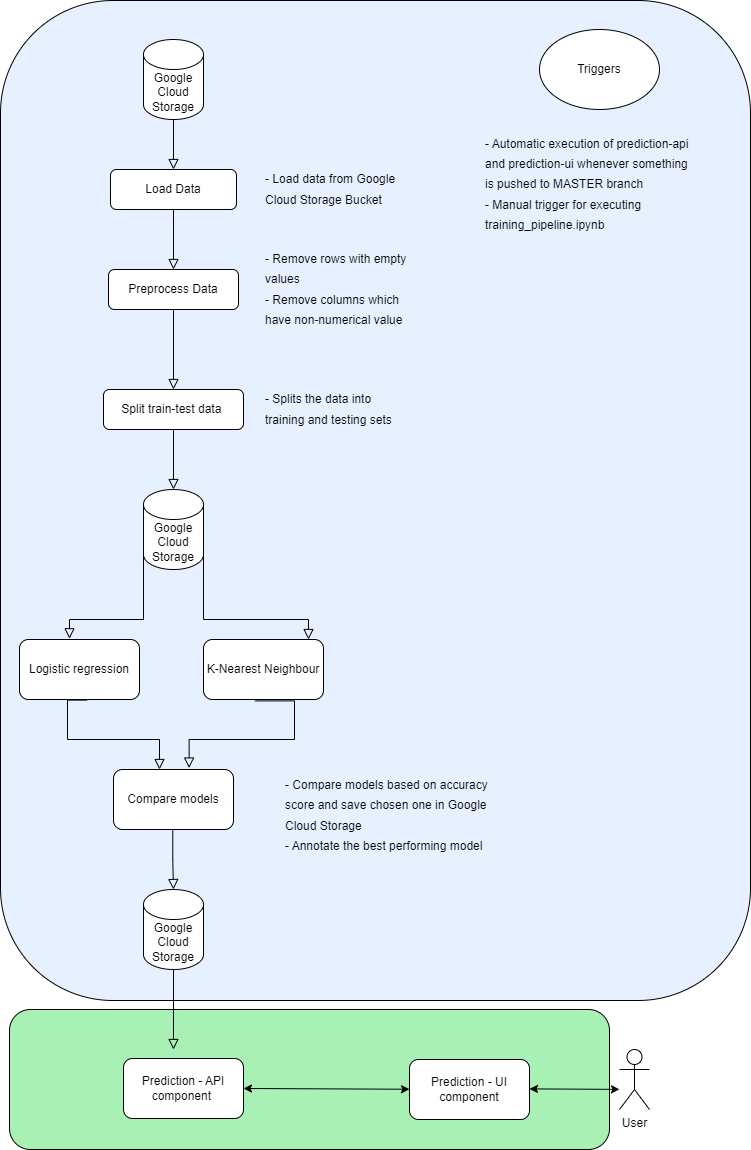
\includegraphics[scale=0.45]{Fig/overview.png}
    \end{center}
\end{wrapfigure}


\end{document}
